\documentclass[11pt]{amsart}
\usepackage{geometry}                % See geometry.pdf to learn the layout options. There are lots.
\geometry{letterpaper}                   % ... or a4paper or a5paper or ... 
%\geometry{landscape}                % Activate for for rotated page geometry
%\usepackage[parfill]{parskip}    % Activate to begin paragraphs with an empty line rather than an indent
\usepackage{graphicx}
\usepackage{subfigure}
\usepackage{amssymb}
\usepackage{epstopdf}
\DeclareGraphicsRule{.tif}{png}{.png}{`convert #1 `dirname #1`/`basename #1 .tif`.png}

\newenvironment{packed_enum}{
\begin{enumerate}
  \setlength{\itemsep}{1pt}
  \setlength{\parskip}{0pt}
  \setlength{\parsep}{0pt}
}{\end{enumerate}}

\title{Catalan Numbers}
\author{Math 300}
%\date{}                                           % Activate to display a given date or no date

\begin{document}
\maketitle
%\section{x}
%\subsection{}

Choose one of the following problems and find some initial data.\\

{\bf  Problem 1}:  Let $s_n$ be the number of n-step staircases that you can construct with $n$-rectangles? Find $s_1$, $s_2$, $s_3$, and $s_4$ by drawing pictures.  See the reverse side for the $n=5$ case.\vfill

{\bf Problem 2}: Let $c_n$ be the number of up-right paths on an $n\times n$ grid that do not pass above the diagonal? Find $c_1$, $c_2$, $c_3$, and $c_4$ by drawing pictures. See the reverse side for the $n=5$ case.\vfill

\pagebreak

  \begin{figure}[htp]
  \begin{center}
    \subfigure{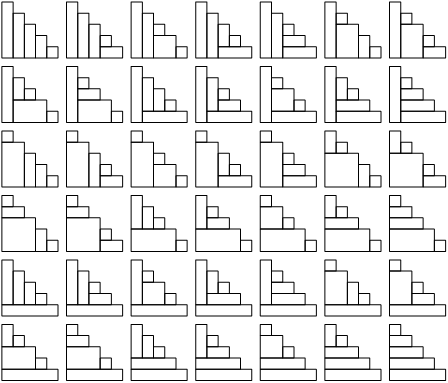
\includegraphics[scale=.60]{Catalan_stairstep_5}}

    \end{center}
\end{figure}
  \begin{figure}[htp]
  \begin{center}

    \subfigure{
\includegraphics[scale=.21]{dyck_path_5}}
    \end{center}
\end{figure}


\end{document}  